\chapter{Diversity}
\label{cp:Diversity}

\section{Species Richness}
A total of 77 bird species were recorded during the period of study. This includes birds from 40 different families.\\
Out of 491 total bird species found in Sri Lanka, this is roughly 15.68\%.

\begin{figure}[!htpb]
    \centering
    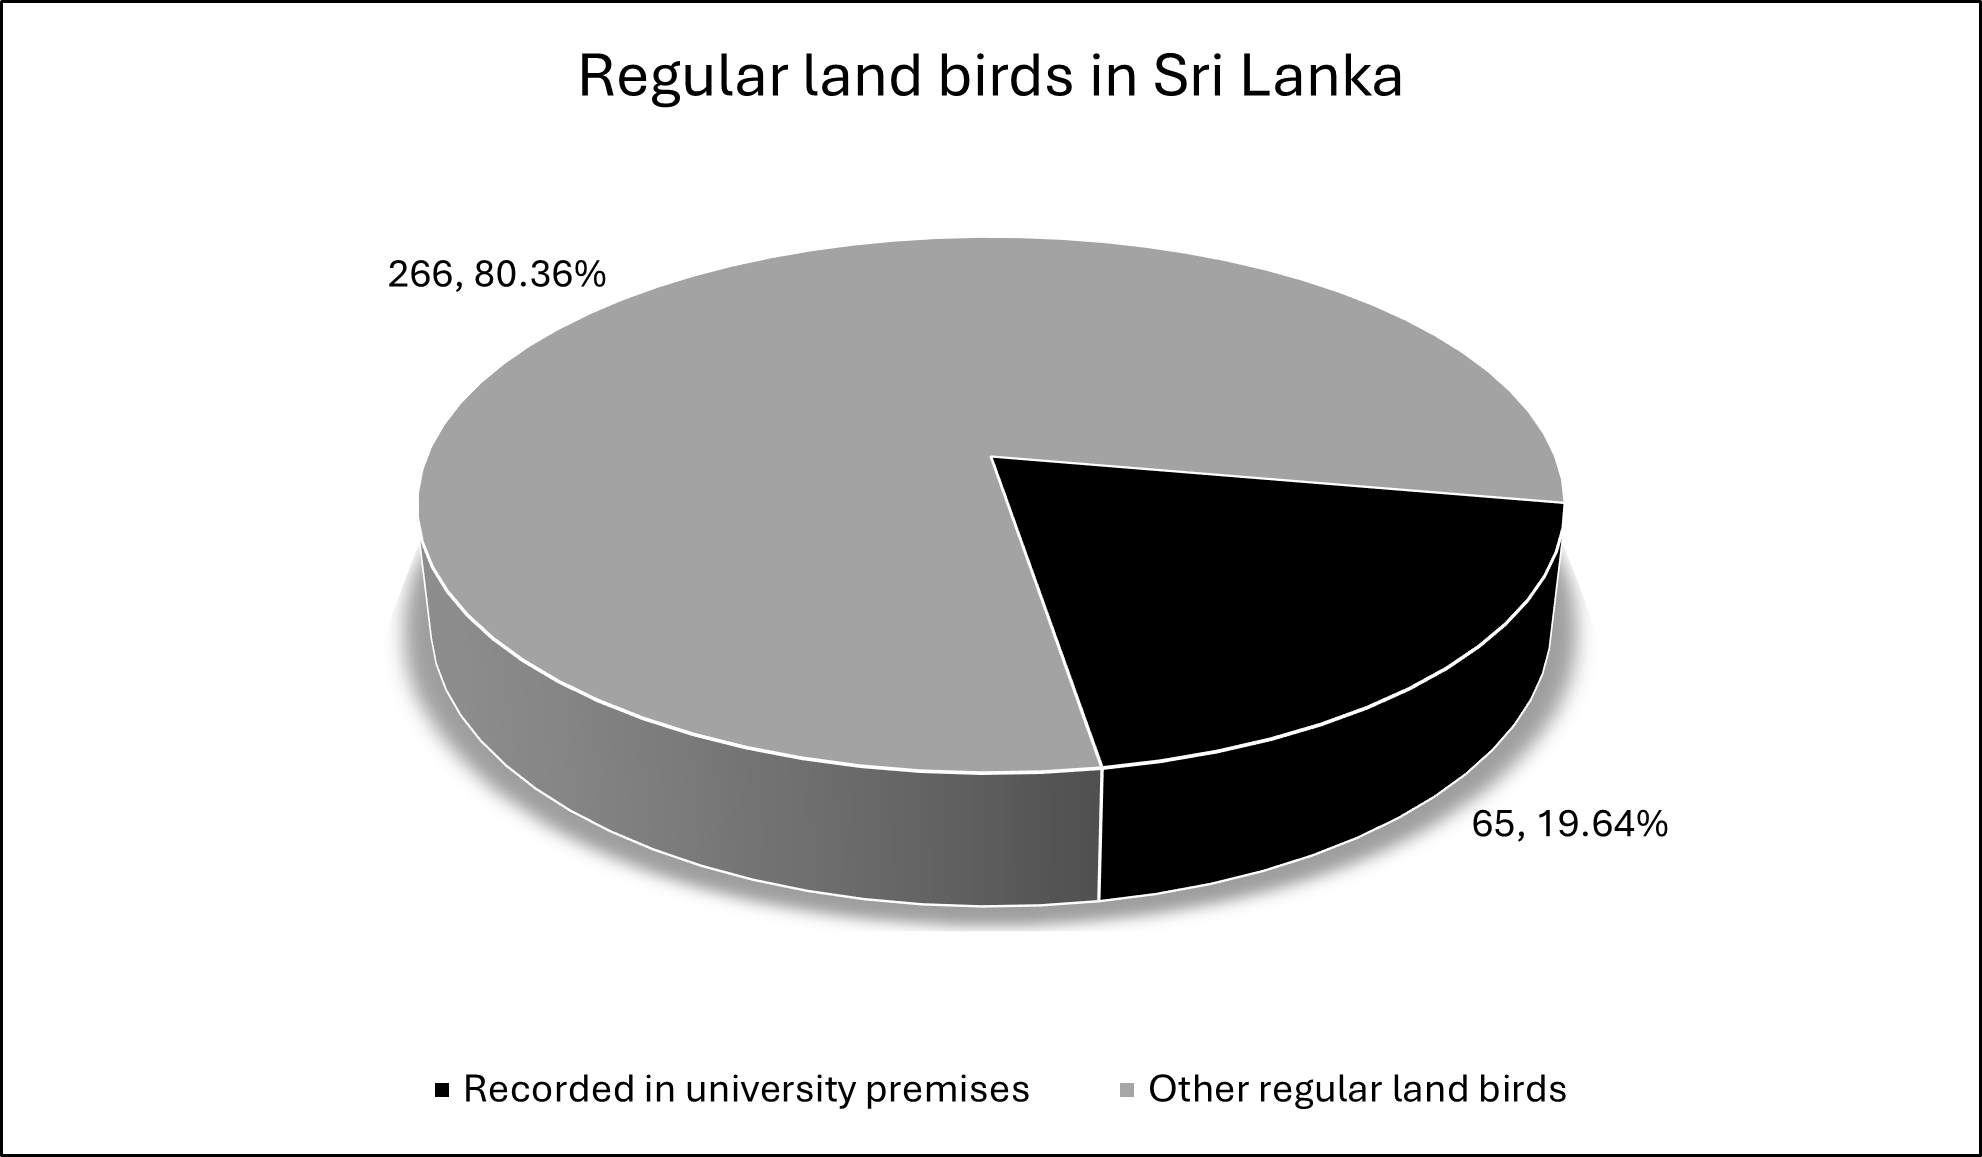
\includegraphics[width=0.9\textwidth]{Figures/pieChart1.png}
    \caption[]{Pie chart showing the recorded number of bird species in the university out of the birds recorded in Sri Lanka.}
    \label{fig:figure-01}
\end{figure}
\noindent 9 out of 77 bird species are migrants to the island while the other 68 species are breeding residents. 

\begin{figure}[!htpb]
    \centering
    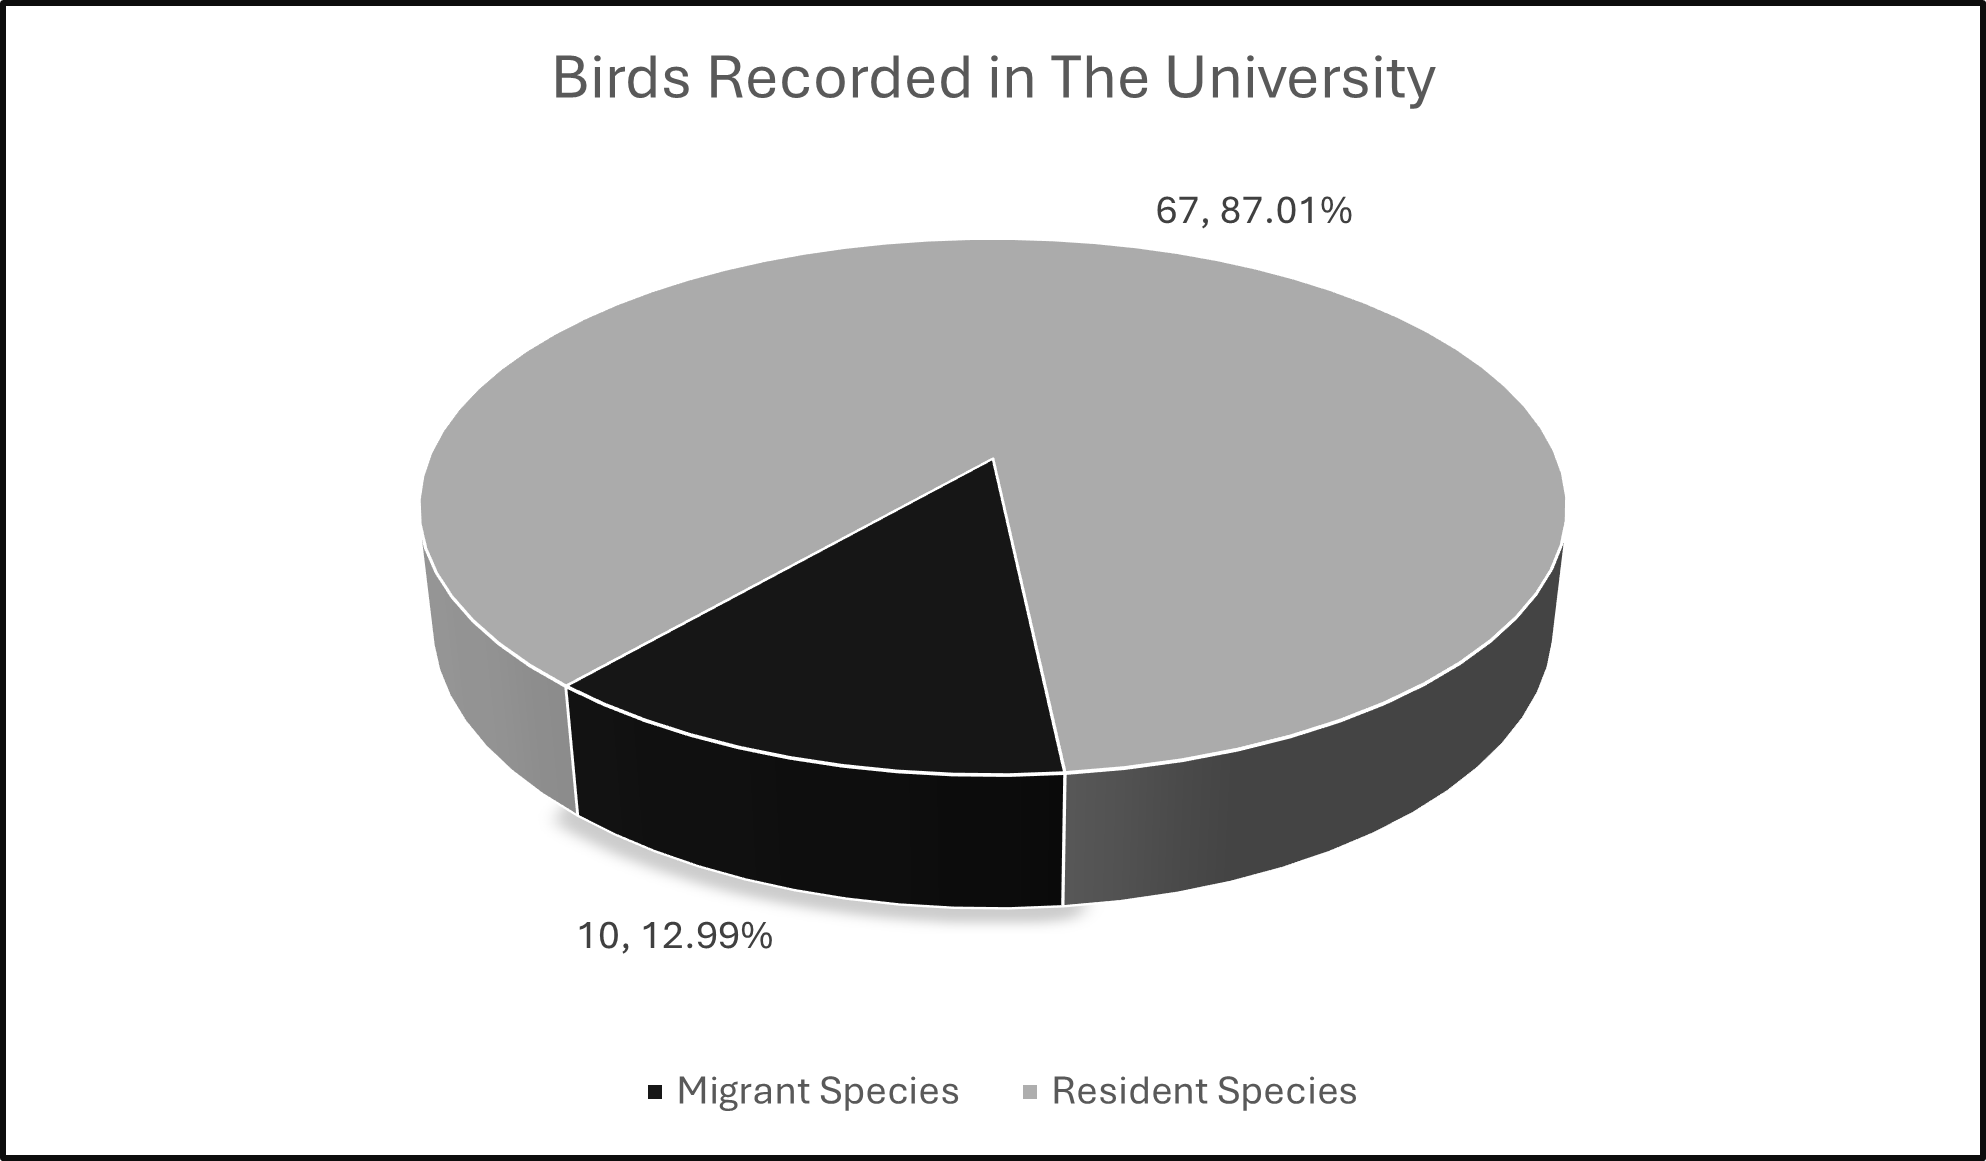
\includegraphics[width=\linewidth]{Figures/pieChart2.png}
    \caption[]{Pie chart showing the number of migrant species and resident species out of total recorded bird species.}
    \label{fig:figure-01}
\end{figure}
\section{Conservation Significance}
The checklist includes single species listed in "Critically Endangered"[3] status and two species listed in "Nearly Threatened"[3] status. Five out of the recorded 77 birds are endemic to Sri Lanka, including,
\begin{itemize}
\item Crimson-fronted Barbet (\textit{Psilopogon rubricapillus})
\item Red{-}Backed Flameback (\textit{Dinopium psarodes})
\item Sri Lanka Green-Pigeon (\textit{Treron pompadora})
 \item Sri Lanka Hanging-Parrot (\textit{Loriculus beryllinus})
   \item Sri Lanka Swallow (\textit{Cecropis hyperythra})
\end{itemize}
Furthermore, the nests of the following bird species were documented.
\begin{itemize}
\item Brahminy Kite (\textit{Haliastur indus})
\item Brown-headed Barbet (\textit{Psilopogon zeylanicus})
\item Purple-rumped Sunbird (\textit{Leptocoma zeylonica})
\item Red-vented Bulbul (\textit{Pycnonotus cafer})
\item Rose-ringed Parakeet (\textit{Psittacula krameri})
\item Scaly-breasted Munia (\textit{Lonchura punctulata})
\item Spotted Dove (\textit{Spilopelia suratensis})
\item Sri Lanka Green-Pigeon (\textit{Treron pompadora})
\item White-bellied Sea Eagle (\textit{Haliaeetus leucogaster})
\item White-rumped Munia (\textit{Lonchura striata})
\end{itemize}
\begin{figure}[!htpb]
    \centering
    \begin{subfigure}{0.45\textwidth}
        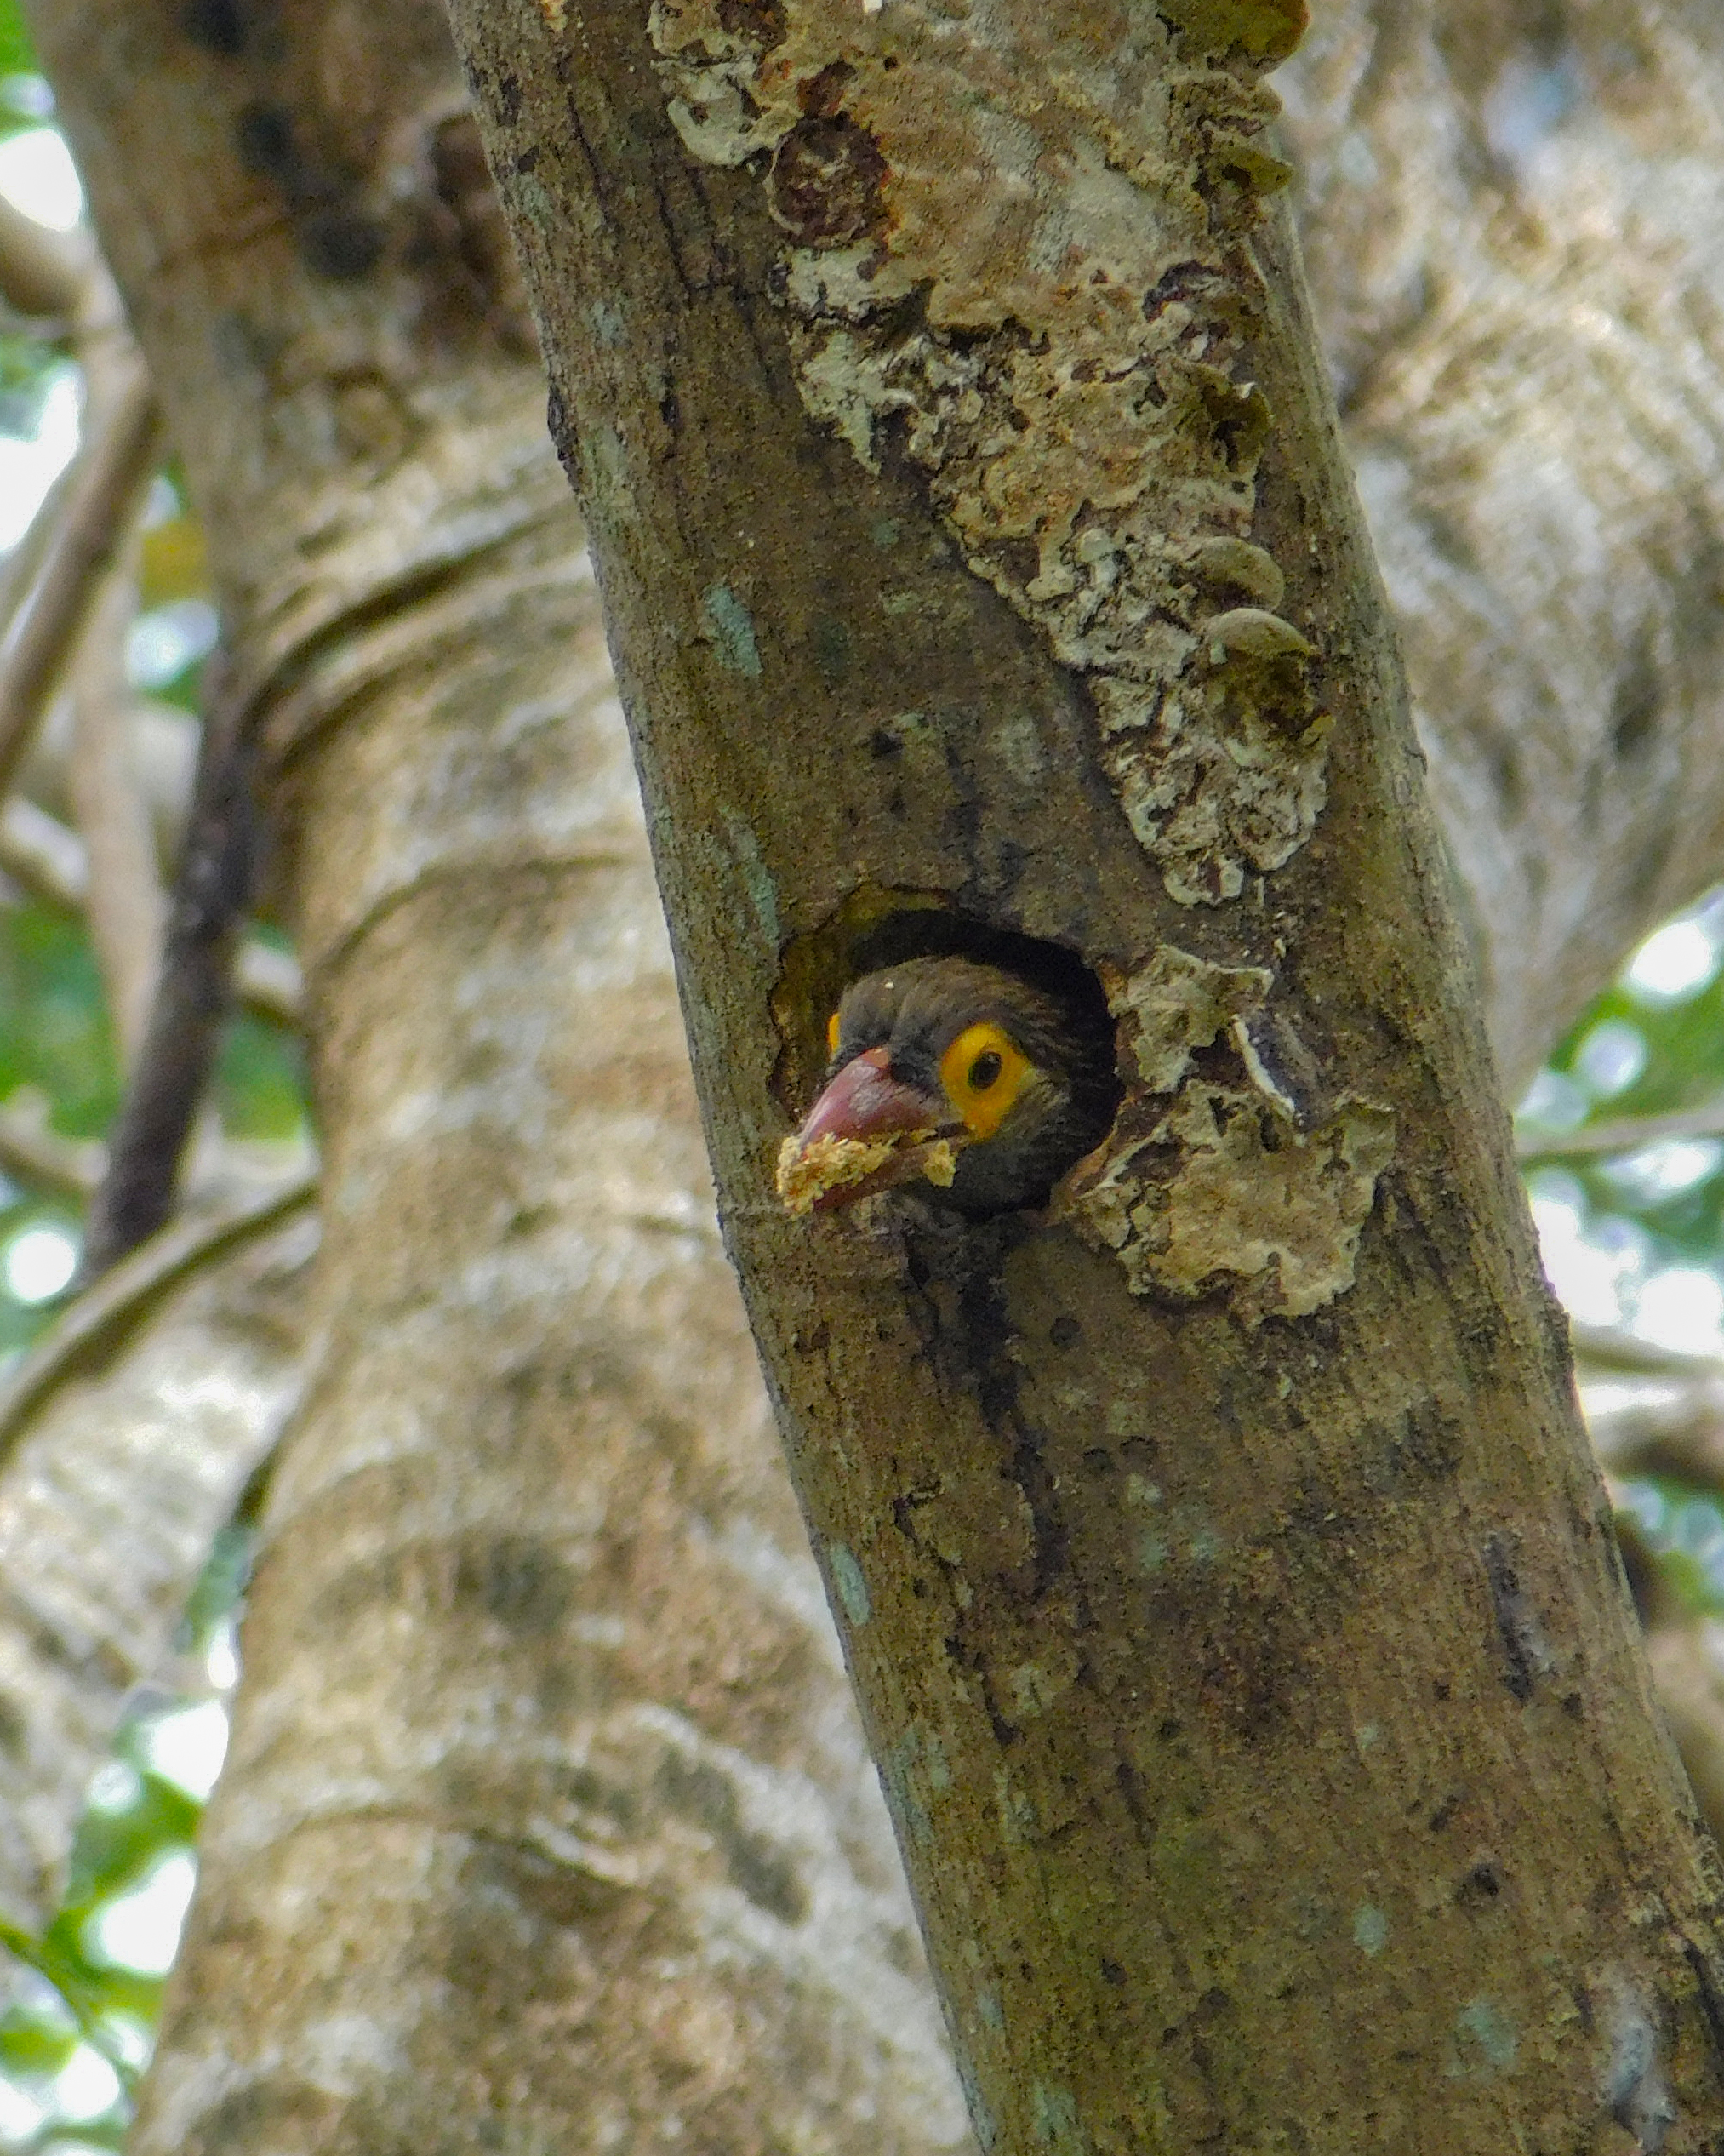
\includegraphics[width=\textwidth]{Figures/brown-headed-barbet.jpg}
        \caption{A Brown-headed Barbet excavating a cavity, Kaju kele.}
        \label{fig:figure-02.1}
    \end{subfigure}
    \hspace{.5cm} % Adjust the space as needed
    \begin{subfigure}{0.45\textwidth}
        \includegraphics[width=\textwidth]{Figures/green-pigeon.jpg}
        \caption{Sri Lanka Green-Pigeon nest near the Dept. of Civil Engineering}
        \label{fig:figure-02.2}
    \end{subfigure}

    
    \begin{subfigure}{0.45\textwidth}
        \includegraphics[width=\textwidth]{Figures/loten's-sun-bird}
        \caption{Purple-rumped Sunbird nest behind the Dept. of Civil Engineering.}
        \label{fig:figure-02.2}
    \end{subfigure}
    \hspace{.5cm} % Adjust the space as needed
    \begin{subfigure}{0.45\textwidth}
        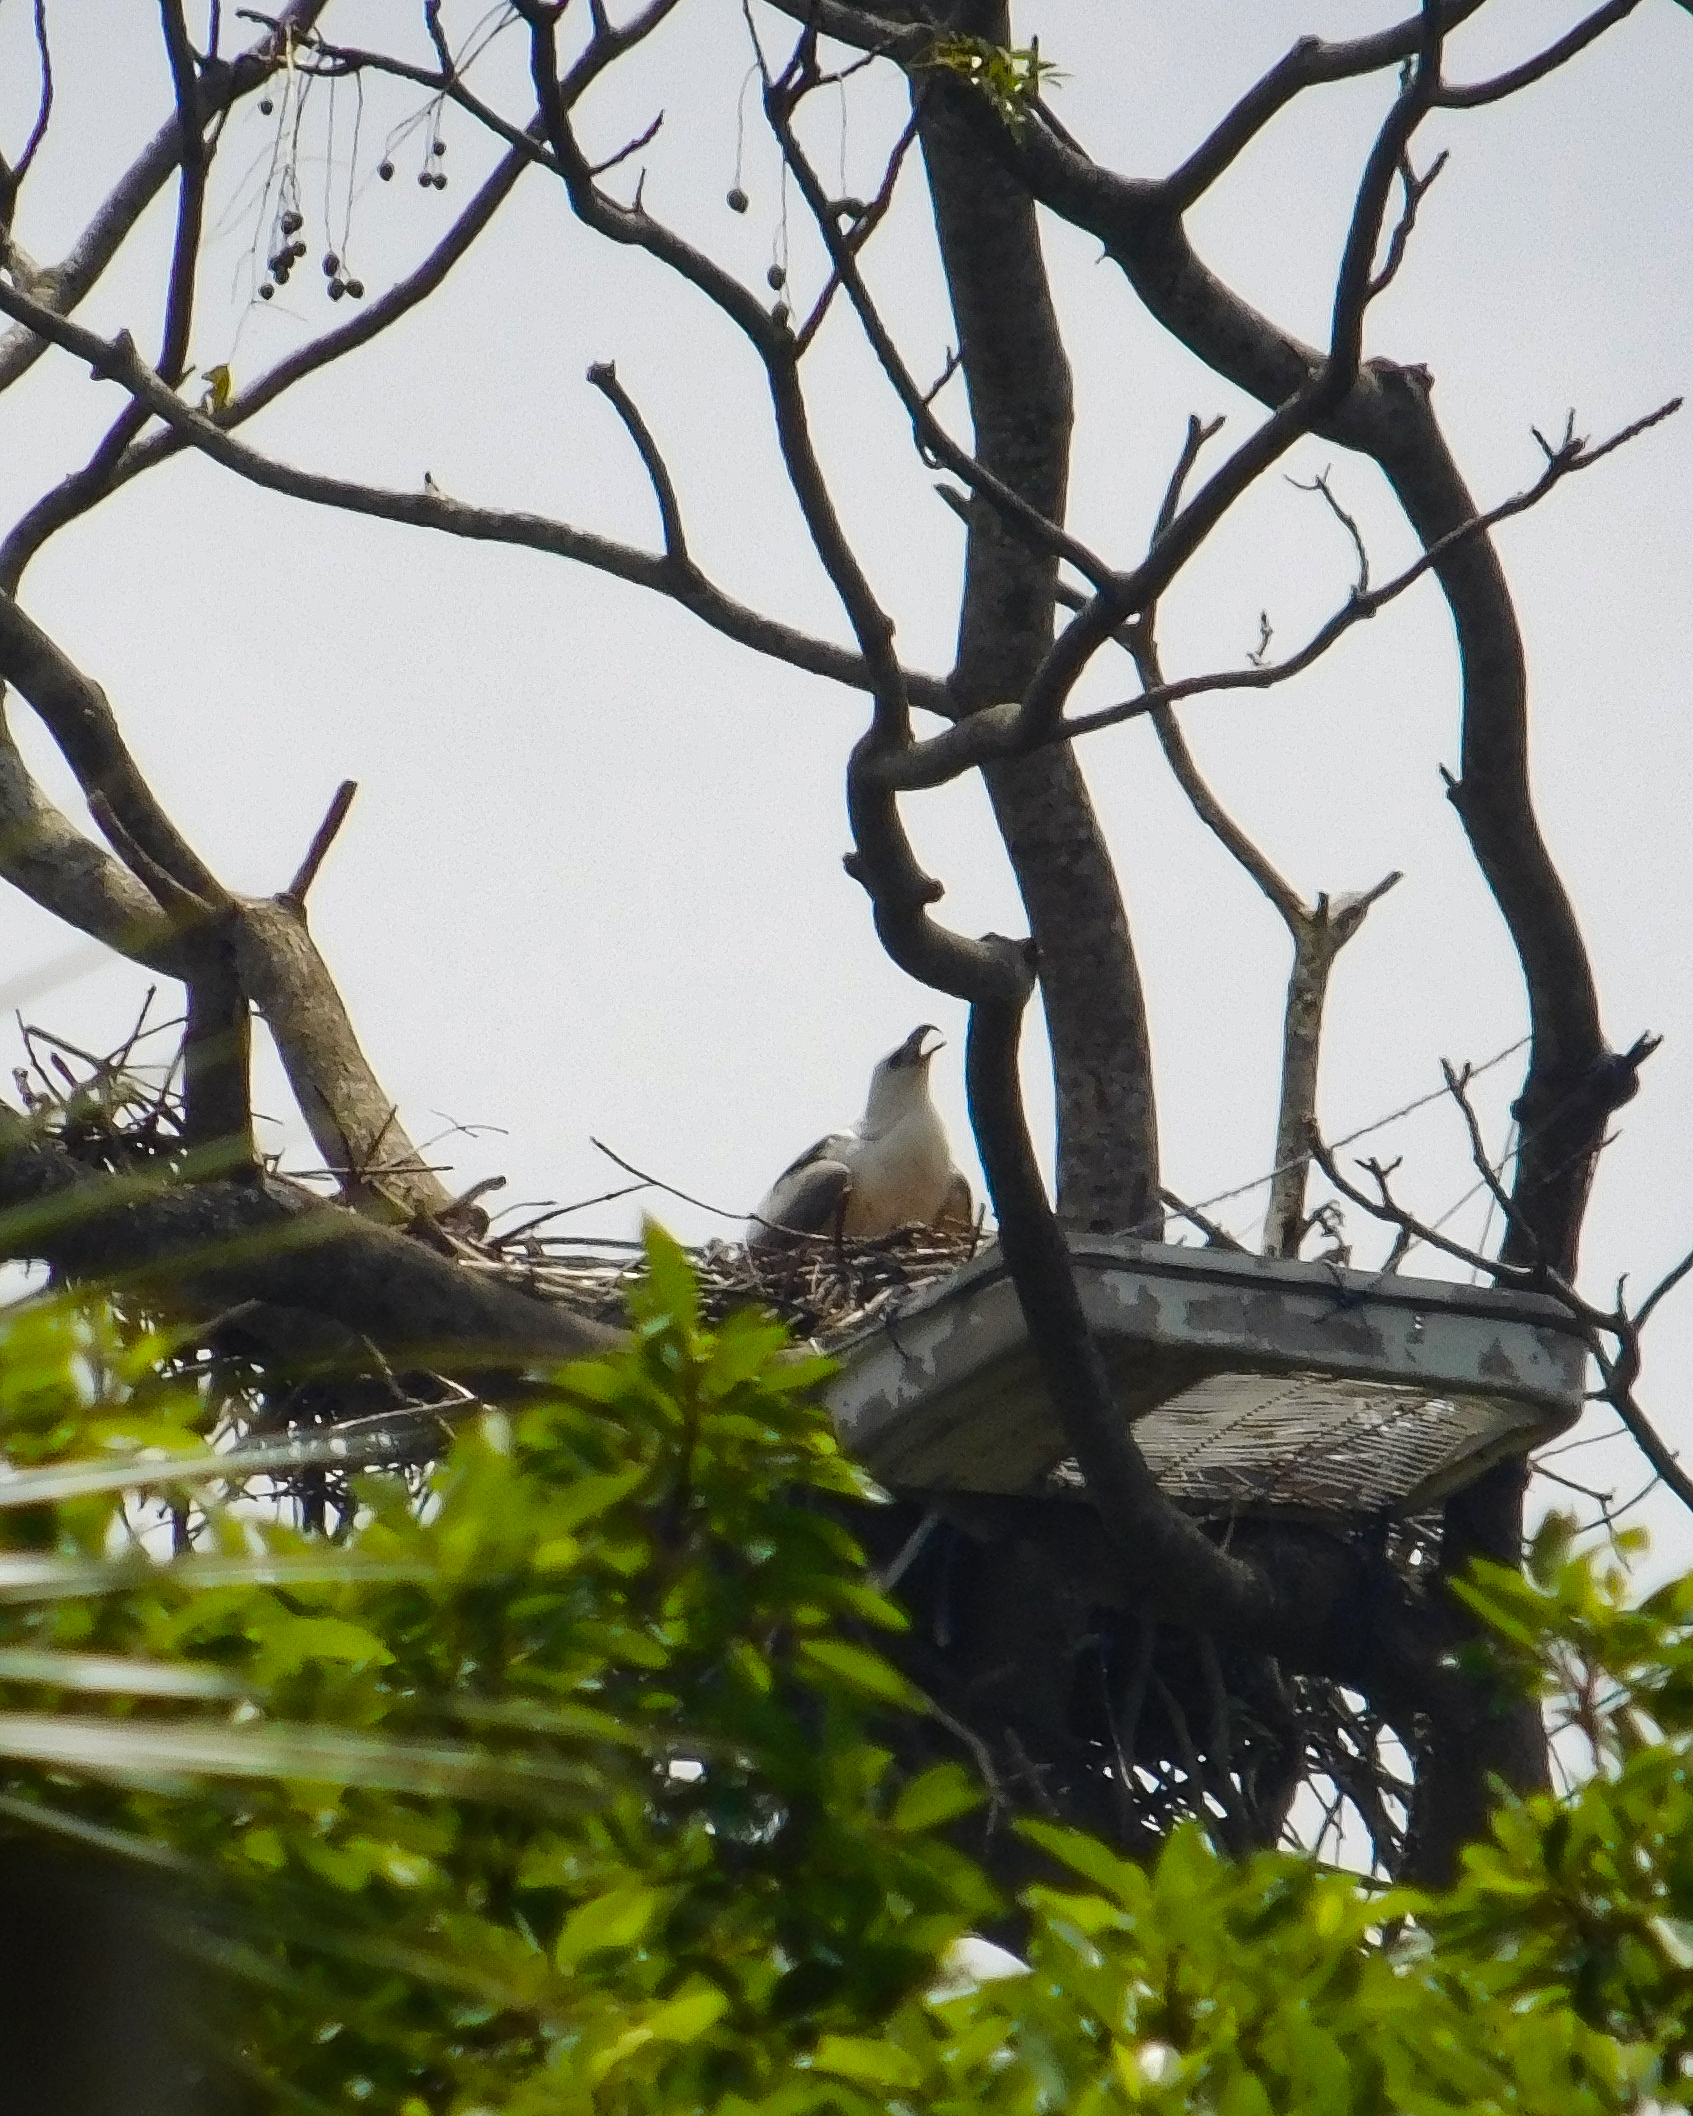
\includegraphics[width=\textwidth]{Figures/white-bellied-sea-eagle.jpg}
        \caption{White-bellied Sea Eagle nest visible to Kaju kele lovers lane.}
        \label{fig:figure-02.2}
    \end{subfigure}
    \caption{Some of the bird nests recorded}
    \label{fig:figure-02}
\end{figure}
% \nameref{cp:citations} (referred to as \autoref{cp:citations}).

\section{Rarity of Species}
While some of the species recorded are very common in the university premises, some others are relatively rare. There were even some species that were recorded only once during the period of study.
\begin{itemize}
    \item Black-winged Stilt (\textit{Himantopus himantopus})
    \item Changeable Hawk-Eagle (\textit{Nisaetus cirrhatus})
    \item Indian Golden Oriole (\textit{Oriolus kundoo})
    \item Indian Robin (\textit{Saxicoloides fulicatus})
    \item Painted Stork (\textit{Mycteria leucocephala})
    
\end{itemize}
falls under this category.
\begin{figure}[!htpb]
    \centering
    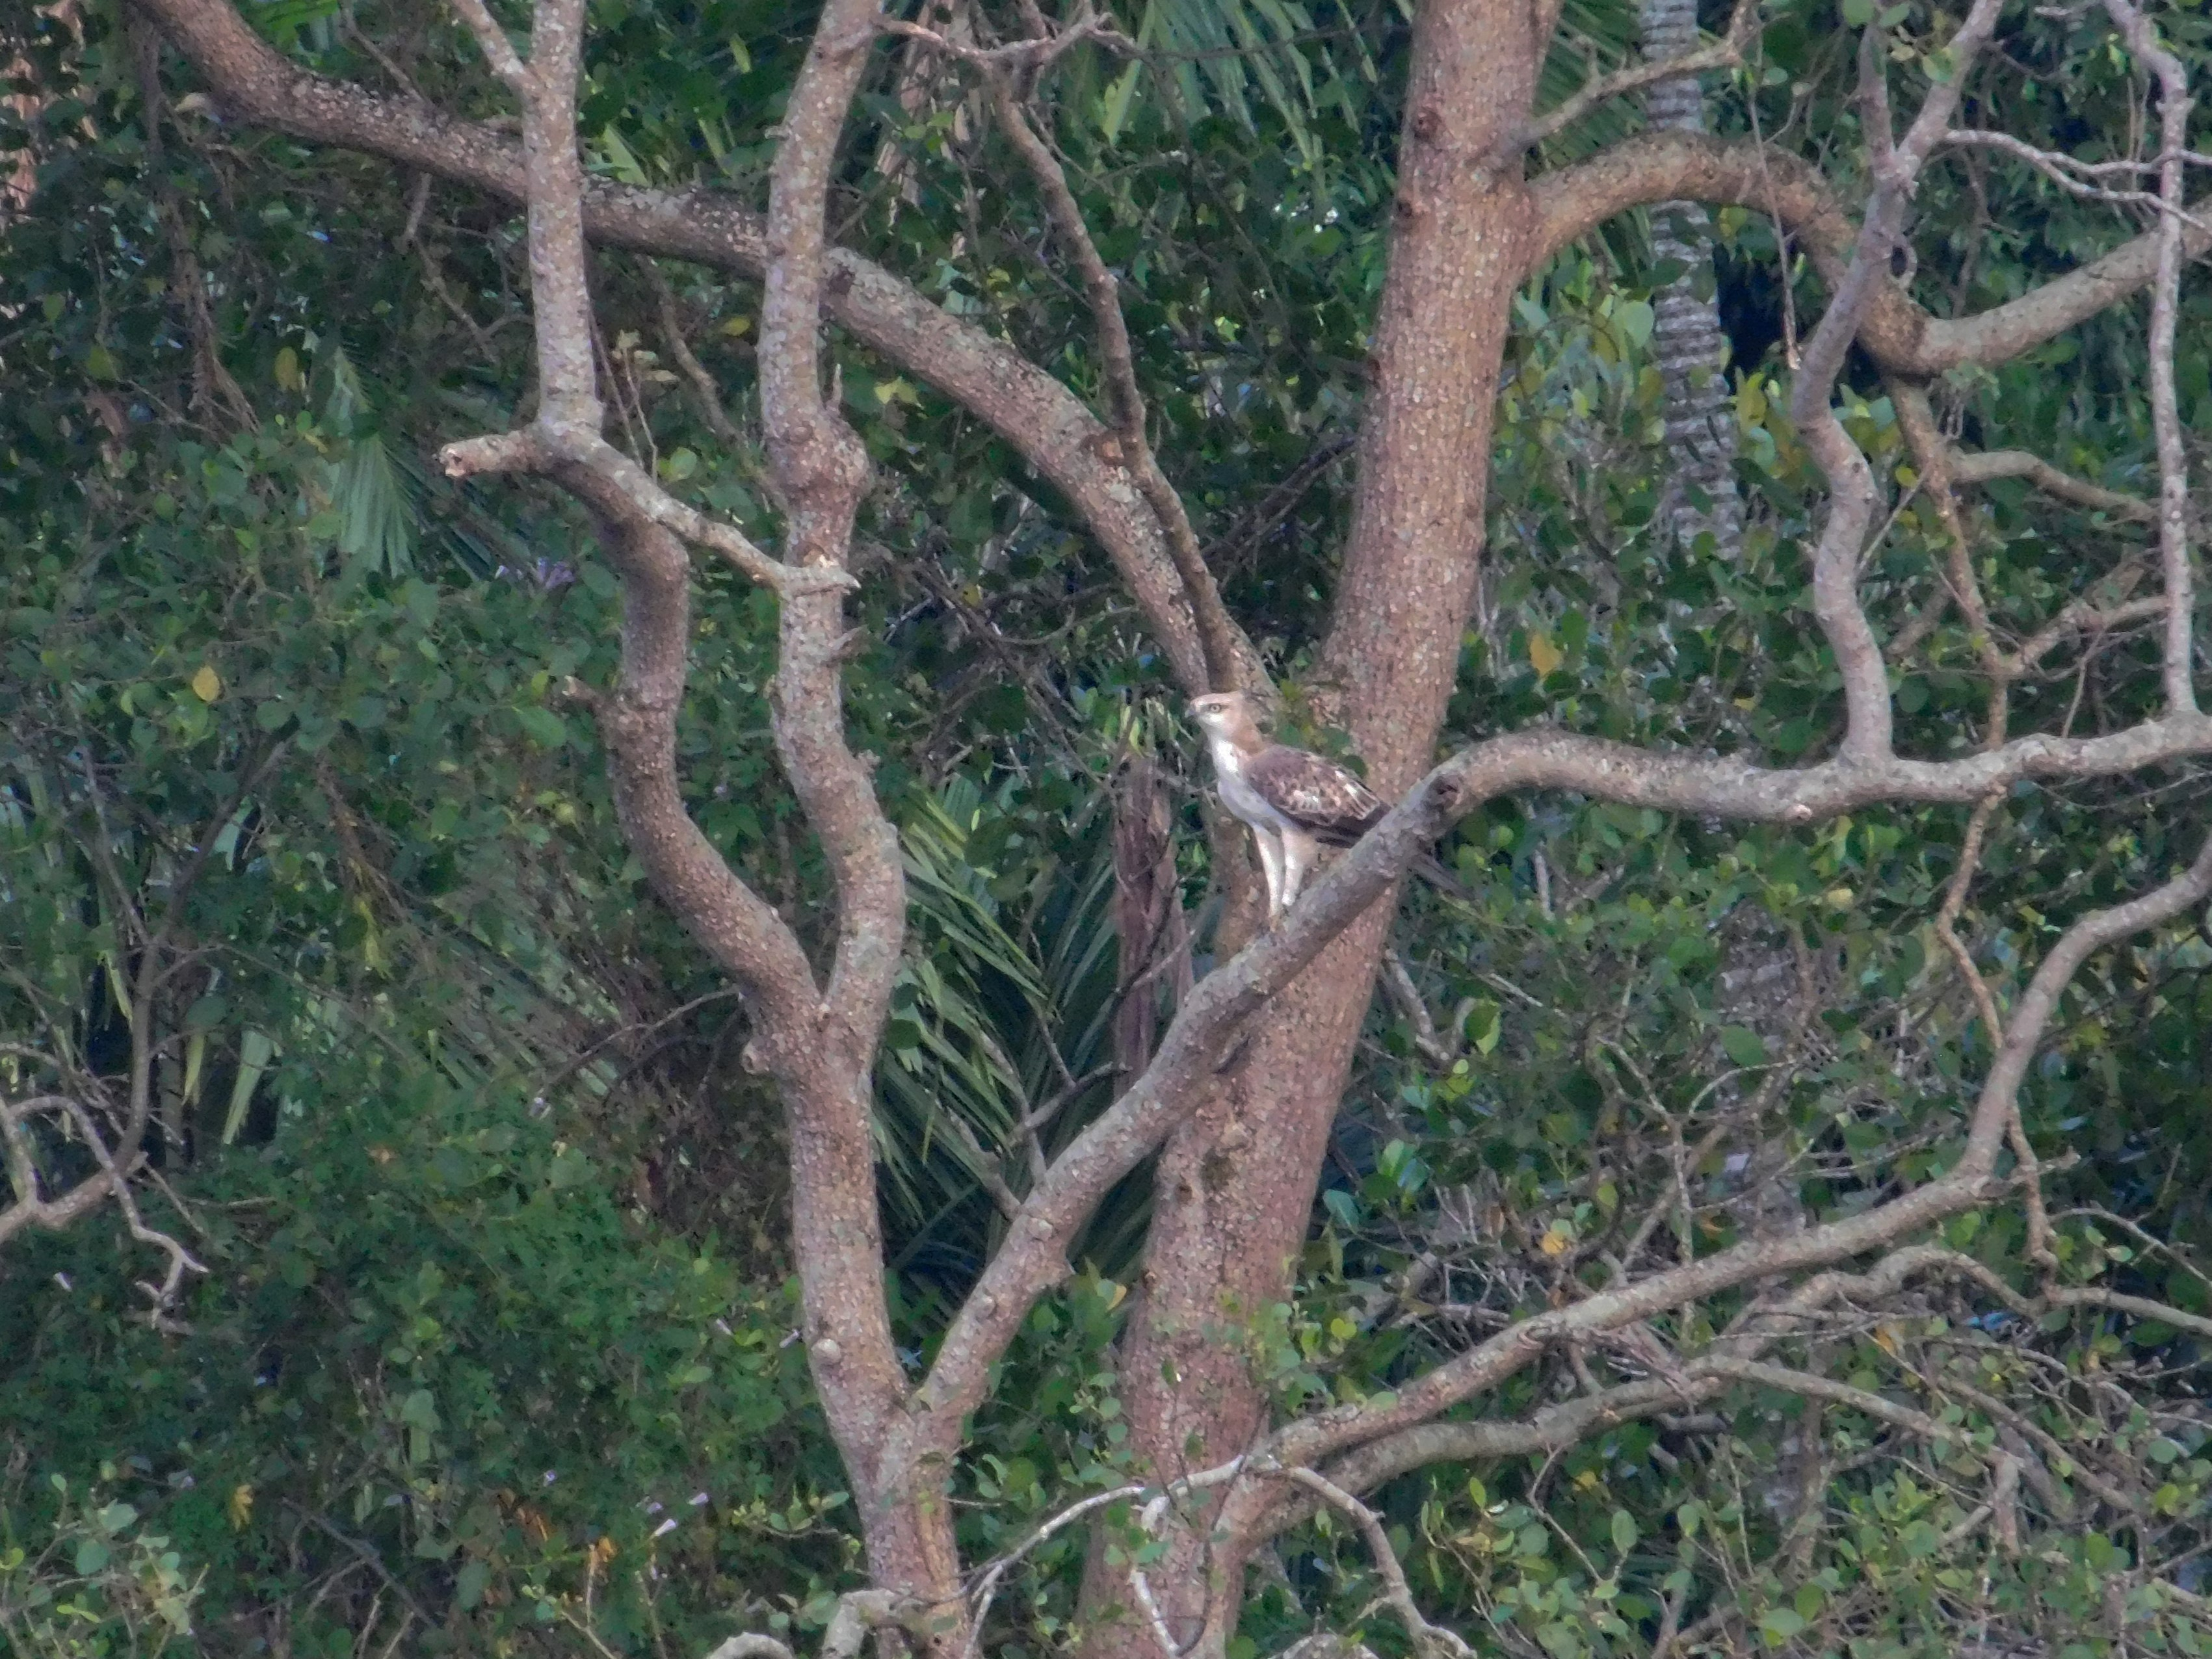
\includegraphics[width=\linewidth]{Figures/crested-hawk.jpg}
    \caption[]{A photograph of the one and only sighting of a Changeable Hawk-Eagle throughout the period of study, taken at boat yard.}
    \label{fig:figure-01}
\end{figure}

